%%%%%%%%%%%%%%%%%%%%%%%%%%%%%%%%%%%%%%%%%
% Thesis Template
% LaTeX Template
% Version 1.0 (29/12/18)
%
%
% This template is based on a template downloaded from:
% http://www.LaTeXTemplates.com
%
% Version 2.x major modifications by:
% Vel (vel@latextemplates.com)
%
% which in turn was based on a template by:
% Steve Gunn (http://users.ecs.soton.ac.uk/srg/softwaretools/document/templates/)
% Sunil Patel (http://www.sunilpatel.co.uk/thesis-template/)
% 
%
% Template license:
% CC BY-NC-SA 3.0 (http://creativecommons.org/licenses/by-nc-sa/3.0/)
%
%%%%%%%%%%%%%%%%%%%%%%%%%%%%%%%%%%%%%%%%%

%-----------
%        PACKAGES AND OTHER DOCUMENT CONFIGURATIONS
%---------------

\documentclass[
12pt, % The default document font size, options: 10pt, 11pt, 12pt
%oneside, % Two side (alternating margins) for binding by default, uncomment to switch to one side
english, % ngerman for German
onehalfspacing, % Single line spacing, alternatives: singlespacing, onehalfspacing or doublespacing
% draft, % Uncomment to enable draft mode (no pictures, no links, overfull hboxes indicated)
nolistspacing, % If the document is onehalfspacing or doublespacing, uncomment this to set spacing in lists to single
liststotoc, % Uncomment to add the list of figures/tables/etc to the table of contents
%toctotoc, % Uncomment to add the main table of contents to the table of contents
%parskip, % Uncomment to add space between paragraphs
%nohyperref, % Uncomment to not load the hyperref package
headsepline, % Uncomment to get a line under the header
]{Thesis} % The class file specifying the document structure

\usepackage[utf8]{inputenc} % Required for inputting international characters
\usepackage[T1]{fontenc} % Output font encoding for international characters
\usepackage{titlesec}
\usepackage{palatino} % Use the Palatino font by default
\usepackage{charter} % Use the Charter font by default

\usepackage[backend=bibtex,style=ieee,natbib=true]{biblatex} % User the bibtex backend with the authoryear citation style (which resembles APA)
\usepackage{epigraph}

\addbibresource{library.bib} % The filename of the bibliography
\DeclareBibliographyCategory{ignore} % for entries that should not appear in the bibliography but are cited

\usepackage[autostyle=true]{csquotes} % Required to generate language-dependent quotes in the bibliography
%\usepackage{afterpage} 

% For adding todos to the text
\usepackage{xcolor} 
\usepackage[author={Your Name}]{pdfcomment}

% For figures in tables to align the vertically
\usepackage{mwe}
\usepackage[export]{adjustbox}

% for the checkmark
\usepackage{amssymb}
\usepackage{pifont}

% Reset link color. For more information and settings:
% http://tex.stackexchange.com/questions/50747/options-for-appearance-of-links-in-hyperref
\hypersetup{
colorlinks = true,
linkcolor = black,
citecolor = gray,
urlcolor = black
}

%----------------------------------------------------------------------------------------
%        MARGIN SETTINGS
%----------------------------------------------------------------------------------------

\geometry{
        paper=a4paper, % Change to letterpaper for US letter
        inner=2.54cm, % Inner margin
        outer=2.8cm, % Outer margin
        bindingoffset=1cm, % Binding offset
        top=2.5cm, % Top margin
        bottom=2.5cm, % Bottom margin
        %showframe,% show how the type block is set on the page
}
\emergencystretch 3em

%----------------------------------------------------------------------------------------
%        THESIS INFORMATION
%----------------------------------------------------------------------------------------

\thesistitle{Building Management: Machine Vision} % Your thesis title, this is used in the title and abstract, print it elsewhere with \ttitle
\supervisor{Prof. Dr.-Ing. Ralph  \textsc{Hänsel}} % Your supervisor's name, this is used in the title page, print it elsewhere with \supname
%\currentYear{} % When you hand it in
\examiner{} % Your examiner's name, this is not currently used anywhere in the template, print it elsewhere with \examname
\degree{Bachelor of Science (B.Sc.)} % Your degree name, this is used in the title page and abstract, print it elsewhere with \degreename
\program{Information Technology} % the programm you are enrolled in
\author{Xinchen \textsc{YANG}} % Your name, this is used in the title page and abstract, print it elsewhere with \authorname
\addresses{} % Your address, this is not currently used anywhere in the template, print it elsewhere with \addressname
\university{Technical University of Applied Sciences Lübeck}
\keywords{} % Keywords for your thesis, this is not currently used anywhere in the template, print it elsewhere with \keywordnames
\pillar{Department of Electrical Engineering and Computer Science} % Pillar

\hypersetup{pdftitle=\ttitle} % Set the PDF's title to your title
\hypersetup{pdfauthor=\authorname} % Set the PDF's author to your name
\hypersetup{pdfkeywords=\keywordnames} % Set the PDF's keywords to your keywords

% Definition how figures, sections tables should be referenced
\usepackage[nameinlink]{cleveref}
\crefname{figure}{Figure}{Figure}
\crefname{section}{Section}{Section}
\crefname{table}{Table}{Table}

%----------------------------------------------------------------------------------------
%        CUSTOMIZED COMMANDS AND ENVIRONMENTS
%----------------------------------------------------------------------------------------

% CHANGE CHAPTER HEADING
%Options: Sonny, Lenny, Glenn, Conny, Rejne, Bjarne, Bjornstrup
\usepackage[Rejne]{fncychap}
%\ChTitleVar{\centering\HUGE\bfseries\selectfont}
\ChNameVar{\centering\small\fontseries{b}\selectfont}
\ChTitleVar{\centering\LARGE\bfseries}
%\ChNameUpperCase, \ChRuleWidth{1pt}
%\ChNumVar{\fontsize{36}{162}\bfseries}
%\ChNameAsIs
%\ChRuleWidth{0.5pt}
%\ChNameUpperCase
%\ChNameVar{\centering\Huge\rm\bfseries}
%\ChNameVar{\fontsize{14}{16}\usefont{OT1}{phv}{m}{n}\selectfont}
%\ChNumVar{\fontsize{60}{62}\usefont{OT1}{ptm}{m}{n}\selectfont} 
%\ChTitleVar{\Huge\bfseries\m} 
\ChRuleWidth{2pt}

\usepackage{threeparttable}
\usepackage{xspace} % for spaces defined commands
\usepackage{textcomp} % for degree symbol
\usepackage{rotating}
\usepackage{needspace}
\usepackage{pdfpages} % to include pdf pages in the appendix
\usepackage{subfigure}
% set counter for numbered sections to 3 so that subsubsections also get a number
\setcounter{secnumdepth}{3}
\setcounter{tocdepth}{2}



% Adjust par indent and skip
\setlength{\parindent}{0pt}
\setlength{\parskip}{12pt plus 2pt minus 2pt}


\makeatletter
\renewcommand{\@chapapp}{}
\newenvironment{chapquote}[2][2em]
  {\setlength{\@tempdima}{#1}%
  \def\chapquote@author{#2}%
  \parshape 1 \@tempdima \dimexpr\textwidth-2\@tempdima\relax%
  \itshape}
{\par\normalfont\hfill--\ \chapquote@author\hspace*{\@tempdima}\par\bigskip}

\newcommand*{\rom}[1]{\expandafter\@slowromancap\romannumeral #1@}
\makeatother

% for global renewcommand
\makeatletter
\def\gnewcommand{\g@star@or@long\new@command}
\def\grenewcommand{\g@star@or@long\renew@command}
\def\g@star@or@long#1{% 
  \@ifstar{\let\l@ngrel@x\global#1}{\def\l@ngrel@x{\long\global}#1}}
\makeatother

%----------------------------------------------------------------------------------------
%        DRAFT MODE
%----------------------------------------------------------------------------------------

\newboolean{isDraft}
\setboolean{isDraft}{false}

%----------------------------------------------------------------------------------------
%        MY OWN COMMANDS
%----------------------------------------------------------------------------------------

% Constants, e.g., initial set of papers for a systematic literature review
\newcommand{\slrainitialset}[0]{1679\xspace}
\newcommand{\slrafinalset}[0]{81\xspace}
\newcommand{\slrpfinalset}[0]{23\xspace}
\newcommand{\slruniquemsss}[0]{77\xspace}


\newcommand{\rqone}[0]{What are important considerations for designing Music Sensory-Substitution Systems that provide an enjoyable music-making experience?}
\newcommand{\rqtwo}[0]{What are the current capabilities, strategies, and challenges of deaf people who are starting to play an instrument?}
\newcommand{\rqthree}[0]{How can all the nontrivial requirements of providing real-time feedback, adaptability, and free limb movement be addressed with a single design?}
\newcommand{\rqfour}[0]{How can technology be used to provide more information about rhythm to a deaf person during a music-making activity?}

\newcommand{\rqcite}[2]{\q{#2} (\textbf{RQ #1})}


% For approximation
\let\oldapprox=\approx 
\renewcommand{\approx}[0] {$\oldapprox$}

% For quotes
\newcommand{\q}[1] {\textit{``#1''}\xspace}

% For subsubsubsections
\newcommand{\subsubsubsection}[1] {
\par
\needspace{1em}
\textit{#1}\\}

% This makes all citations' authors gray
% Also see \hypersetup{citecolor} !
\let\oldcite=\citealp 
\renewcommand{\citep}[2][]{(\textcolor{gray}{\oldcite[#1]{#2}})}

% to avoid that big figures directly get their own page
\renewcommand{\floatpagefraction}{.8}

% Creates the label for a chapter
% Param1: label for the appendix
\newcommand{\chaplabel}[1]{\label{ch:#1}}

% Creates the reference for an appendix
% Param1: label of the appendix
\newcommand{\chapref}[1]{Chapter~\ref{ch:#1}}

% Creates the label for an appendix
% Param1: label for the appendix
\newcommand{\alabel}[1]{\label{app:#1}}

% Creates the reference for an appendix
% Param1: label of the appendix
\newcommand{\aref}[1]{Appendix~\ref{app:#1}}

% Creates an appendix header
% Param1: label of the appendix
\newcommand{\aheader}[2]{\section{#1}\alabel{#2}}

% Creates the label for a section 
% Param1: name for the section
\newcommand{\seclabel}[1]{\label{sec:\thechapter:#1}}

% Creates the reference for a section 
% Param1: (optional) chapter
% Param2: name of the section
\newcommand{\secref}[2][\thechapter]{\cref{sec:#1:#2}}

% Creates the reference for a figure 
% Param1: (optional) chapter
% Param2: name of the figure
% Param3: subfigure, e.g. a, b, c
% e.g.: \fref[1]{feedbackloop}{} - if you are outside chapter 1 without subfigure
% \fref{feedbackloop}{a} - if you are inside chapter 1 with reference to subfigure a
\newcommand{\fref}[3][\thechapter]{\cref{fig:#1:#2}#3\xspace}


% Param1: (optional) width of the figure in relation to \textwidth
% Param2: figure name
% Param3: caption
% Param4: label name
% Usage: \finsert[0.6]{feedback-loop}{Here you see a feedback loop}{feedbackloop}
\newcommand{\finsert}[4][1]{
\begin{figure}[t]
\centering
\includegraphics[width=#1\textwidth]{#2}
\caption{#3}\label{fig:\thechapter:#4}
\end{figure}
}

% Same as \finsert just that the figure will be placed at point of insert
\newcommand{\fhere}[4][1]{
\begin{figure}[ht]
\centering
\includegraphics[width=#1\textwidth]{#2}
\caption{#3}\label{fig:\thechapter:#4}
\end{figure}
}



% Is used by fancytable environment
\newenvironment{nstabbing}
{\setlength{\topsep}{0pt}
\setlength{\partopsep}{0pt}
\tabbing}{\endtabbing}
\newcommand{\fancytablecaption}[0]{}
\newcommand{\fancytablecitestring}[0]{}
\newcommand{\fancytablestretchvalue}[0]{1.5}
\newcommand{\fancytablecaptionstring}[0]{}
\newcommand{\fancytablestretch}[1]{\renewcommand{\fancytablestretchvalue}[0]{#1}}
\newcommand{\fancytablelegend}[1]{\renewcommand{\fancytablecitestring}[0]{#1}}

% \end{fancytable}
\newenvironment{fancytable}[5][1]
{
  \grenewcommand{\fancytablecaption}[0]{\caption{#3}\label{tab:\thechapter:#4}}

\begin{table}[!htb]
  \footnotesize
  \centering
  \def\arraystretch{\fancytablestretchvalue}
  \begin{tabular*}{#1\textwidth}{#2}
    \hline
      #5\\
    \hline
}
{
    \hline
  \end{tabular*}
\ifx&\fancytablecitestring&%

\else
\begin{nstabbing}
  \fancytablecitestring
\end{nstabbing}
\fi
  \fancytablecaption
\grenewcommand{\fancytablecitestring}[0]{}
\grenewcommand{\fancytablestretchvalue}[0]{1.5}
\end{table}
}

% Is used by fancytable environment

\newcommand{\fancytablecaptionz}[0]{}
\newcommand{\fancytablecitestringz}[0]{}
\newcommand{\fancytablestretchvaluez}[0]{1.5}
\newcommand{\fancytablecaptionstringz}[0]{}
\newcommand{\fancytablestretchz}[1]{\renewcommand{\fancytablestretchvaluez}[0]{#1}}
\newcommand{\fancytablelegendz}[1]{\renewcommand{\fancytablecitestringz}[0]{#1}}

\newenvironment{fancytablez}[5][1]
{
  \ifx&#3&%
\grenewcommand{\fancytablecaptionz}[0]{\caption{\fancytablecaptionstringz~(cont.)}}
\addtocounter{table}{-1}
\else
  \grenewcommand{\fancytablecaptionstringz}[0]{#3}
  \grenewcommand{\fancytablecaptionz}[0]{\caption{#3}\label{tab:\thechapter:#4}}
\fi

\begin{table}[!htb]
  \footnotesize
  \centering
  \def\arraystretch{\fancytablestretchvaluez}
  \begin{tabular*}{#1\textwidth}{#2}
    \hline
      #5\\
    \hline
}
{
    \hline
  \end{tabular*}
\ifx&\fancytablecitestringz&%

\else
\begin{nstabbing}
  \fancytablecitestringz
\end{nstabbing}
\fi
  \fancytablecaptionz
\end{table}
}

% Creates the reference for a table 
% Param1: (optional) chapter
% Param2: name of the table
\newcommand{\tref}[2][\thechapter]{\cref{tab:#1:#2}}

% Command to define how a footcite should look like
% Param1: citation name
\renewcommand{\footcite}[1]{\footnote{\citefield{#1}{title}. \citeurl{#1}. Last accessed on \citefield{#1}{urlday}/\citefield{#1}{urlmonth}/\citefield{#1}{urlyear}.}}

% Commands to add todos, things I have to change and revision to the document as pdf commands
% if the boolean ``isDraft'' is set to false, those comments will be omitted!

% Param1: the reference to add, may be empty
\newcommand{\addref}[1]{
\pdfmarkupcomment[markup=Highlight,color=yellow]{(ref)}{Todo: add reference(s): #1}
}

% Param1: comment that describes the todo
\newcommand{\todo}[1]{
\pdfcomment[color=yellow,icon=Comment]{#1}
}

% Param1: comment that describes what to add later
\newcommand{\addlater}[1]{
\pdfmarkupcomment[markup=Highlight,color=yellow]{[...]}{#1}
}

% Param1: text that has to be changed later
\newcommand{\changelater}[1]{
\pdfmarkupcomment[markup=Highlight,color=yellow]{#1}{Change later}
}

% Param1: text that has to be changed later
% Param2: comment that describes what to change
\newcommand{\change}[2]{
\pdfmarkupcomment[markup=Highlight,color=yellow]{#1}{#2}
}

% Param1: text that has to be revised
% Param2: comment that describes what or how to revise
\newcommand{\revise}[2]{
\pdfmarkupcomment[markup=StrikeOut,color=red]{#1}{#2}
}

% redefines all todo commands to NOT add comments in case this is the final version
\ifthenelse{\boolean{isDraft}}{}
{
\renewcommand{\todo}[1]{}
\renewcommand{\addref}[1]{}
\renewcommand{\addlater}[1]{}
\renewcommand{\changelater}[1]{#1}
\renewcommand{\change}[2]{#1}
\renewcommand{\revise}[2]{#1}
}

%--------------------------------------------------------------------------
%        THESIS CONTENT - COVER
%---------------------------------------------------------------------------------
\begin{document}

\frontmatter % Use roman page numbering style (i, ii, iii, iv...) for the pre-content pages
\pagestyle{plain} % Default to the plain heading style until the thesis style is called for the body content

%----------------------------------------------------------------------------------------
%        TITLE PAGE
%----------------------------------------------------------------------------------------

\begin{titlepage}
\begin{center}

\begin{figure}
\centering

\includegraphics[width=0.35\textwidth]{Figures/Logo_TH_Luebeck_new}
\end{figure}

 \hfill\break\\[0cm]
 
{\LARGE \bfseries \ttitle}\\[1.5cm] % Thesis title


Submitted by\\[0.5cm]
\authorname % Author name - remove the \href bracket to remove the link

\vspace{2.3em}

Thesis Advisor\\[0.5cm]
\supname % Supervisor name - remove the \href bracket to remove the link 
 
\vspace{2.3em} 
\textsc{
\programname\\
\pillarname\\
\universityname}\\[1.5cm] % Research group name and department name
 
{A thesis submitted in fulfillment of the requirement to the degree\\\degreename}\\[1.7cm] % University requirement text

 
\the\year{}\\ % Date

\vfill
\end{center}
\end{titlepage}

%----------------------------------------------------------------------------------------
%        DECLARATION PAGE
%----------------------------------------------------------------------------------------

\begin{declaration}
\addchaptertocentry{\authorshipname}

\noindent I, \authorname, declare that this thesis titled, \enquote{\ttitle} and the work presented in it are my own. I confirm that:

\begin{itemize} 
\item This work was done wholly or mainly conducted while in candidature for a degree at \universityname{}.
\item Where any part of this thesis has previously been submitted for a degree or any other qualification at this University or any other institution, this has been clearly stated.
\item Where I have consulted the published work of others, this is always clearly attributed.
\item Where I have quoted from the work of others, the source is always given. With the exception of such quotations, this thesis is entirely my own work.
\item I have acknowledged all main sources of help.
\item Where the thesis is based on work done by myself jointly with others, I have made clear exactly what was done by others and what I have contributed myself.\\
\end{itemize}
 
\noindent Signed:\\
\rule[0.5em]{25em}{0.5pt} % This prints a line for the signature
 
\noindent Date:\\
\rule[0.5em]{25em}{0.5pt} % This prints a line to write the date
\end{declaration}

\cleardoublepage


%----------------------------------------------------------------------------------------
%        ABSTRACT PAGE
%----------------------------------------------------------------------------------------

\begin{abstract}
\addchaptertocentry{\abstractname} % Add the abstract to the table of contents
\noindent International students face the challenge to write a thesis at the end of their studies. As many rules and examples of theses at the Technische Hochschule Lübeck are available in German exclusively they are not suited for the international students. Although many good guidelines are available online they do not cover the specialties of the Technische Hochschule Lübeck. Therefore, a special guideline is necessary. Besides very specific rules for this university some common mistakes are covered in this guideline.

\noindent The task for this work is:
\begin{enumerate}
\item Collection of the German guidelines and existing examples of successful thesis documents.
\item Analysis of the important rules and common mistakes of students when writing an English thesis.
\item	Creation of a comprehensive document serving as a template and a guideline for the students.
\item	Prepare a comprehensive Questions and Answers section.
\end{enumerate}

\noindent The deliveries are:
\begin{itemize}
\item A document that is well structured and serves as a guideline and template
\item A list of frequently asked questions + answers
\end{itemize}
\end{abstract}

%----------------------------------------------------------------------------------------
%        ACKNOWLEDGEMENTS
%----------------------------------------------------------------------------------------

\begin{acknowledgements}
% Add the acknowledgements to the table of contents
\addchaptertocentry{\acknowledgementname}
Put your acknowledgements here! This is an example:
    
    \paragraph{Acknowledgments by Horst Hellbrück}
    I want to thank all staff members and students that have participated in this document by giving tips or by asking questions. When I have started this guide in 2009 with a vague idea in mind, I could not foresee that this document becomes such a great help for all the students. My special thanks go to Zhi Haolin and Ren Zhong from the international study program \programname{} at \universityname{} together with ECUST in Shanghai. They have written most of the texts and provided references and figures. Without their valuable contribution this guide would have stayed at a conceptual level.
    
    \paragraph{Acknowledgements by Ren Zhong}
    I would like to express my gratitude to Prof. Dr.-Ing Horst Hellbrück, who wrote the first draft of this document, and offered me such a great opportunity to contribute to this meaningful work.
    
    \paragraph{Acknowledgements by Andreas Hanemann}
    I would like to thank the people who have worked on this document earlier (Horst Hellbrück, Zhi Haolin, Aida Bahta, Ren Zhong). Some advice from Hermann Hochhaus and Hans-Günter Kunze has also been included into the document.
    
    \paragraph{Acknowledgements by Denys Matthies}
    I would like to particularly thank Martin Ochoa, Vel, Johannes Böttcher, Steve Gunn, Sunil Patand, and Benjamin Petry for providing the basis for this new layout. Thank you!
    
    \paragraph{} The authors hope that students can benefit from the document and that more students may add contributions to this document to improve it.


\end{acknowledgements}

%----------------------------------------------------------------------------------------
%        LIST OF CONTENTS/FIGURES/TABLES PAGES
%----------------------------------------------------------------------------------------

\tableofcontents % Prints the main table of contents

\listoffigures % Prints the list of figures

\listoftables % Prints the list of tables

%----------------------------------------------------------------------------------------
%        ABBREVIATIONS
%----------------------------------------------------------------------------------------

\begin{abbreviations}{ll} % Include a list of abbreviations (a table of two columns)

\textbf{CI} & \textbf{C}ochlea \textbf{I}mplant\\
\textbf{DMI} & \textbf{D}igital \textbf{M}usic \textbf{I}nstrument\\
\textbf{HCI} & \textbf{H}uman \textbf{C}omputer \textbf{I}nteraction\\

\end{abbreviations}


%----------------------------------------------------------------------------------------
%        DEDICATION
%----------------------------------------------------------------------------------------

\dedicatory{Dedicated to my someone,\\who you really appreciate to have in your life.}



%--------------------------------------------------------------------------
%        THESIS CONTENT - CHAPTERS
%---------------------------------------------------------------------------------

\mainmatter % Begin numeric (1,2,3...) page numbering
\pagestyle{thesis} % Return the page headers back to the "thesis" style


\chapter{Introduction}\chaplabel{1}

Building management is one key aspect of facility management. It integrates various disciplines to ensure the functionality, comfort, safety, and efficiency of the building environment for people, processes, and technology. Energy management has become the major aspect of building management nowadays. The calculation of energy consumption of a building is heavily influenced by windows and their roller shutters: while windows emit most of the heat generated by sunlight to the environment, the roller shutters may have a huge impact on such transfer process. In order to optimize the energy consumption of the building, efficient automated building management and monitoring should incorporate available information of the building status. This includes the window status and the roller shutter positions.

 This bachelor thesis aims to investigate and implement in machine vision algorithm for detection of the roller shutter status. Since the estimation of energy consumption is a continuous process, the implemented algorithm should be capable of accurate detection 24/7 and under various weather conditions. In this bachelor thesis, deep learning algorithm You only look once (YOLO) is selected to solve this object detection problem. The detection model is trained and tested via a limited data set obtained manually or by preset cameras on the THL campus.

 This bachelor thesis is organized into three parts. The first part (Chapter 2-4) is a literature review. In Chapter 2, several common solutions are systematically introduced, which includes computer vision, machine learning and Convolutional Neural Networks (CNNs). Chapter 3 explains the applications of CNNs on object detection and main features of YOLO algorithm. Chapter 4 analyzes the existing challenges in roller shutter detection under the requirements of this dissertation.


\chapter{Review of Methodology}\chaplabel{2}

This chapter aims to conduct a preliminary task analysis and paper review, then a systematic introduction to possible methods for solving the given task is provided. A literature review on common methods will be presented to provide a comprehensive understanding of the topic.

\section{Related Work}

The detection of the roller shutters can surely be realized by human eyes and manual measurement. However, different lighting and weather conditions, for example, during the night or on rainy days, may have a huge impact on the preciseness of human eye recognition. In addition, it may cost a lot of time and labor to realize round-the-clock detection. To improve efficiency and reduce costs, previous studies have suggested the use of computers to replace humans in some aspects of these visual tasks, that is, the introduction of \textbf{machine vision}.

Few previous studies focused exactly on detecting the roller shutters of windows. However, as the principles and detection requirements are similar to many other parts of a building, candidate methods for this bachelor thesis can be referenced from studies that aimed to detect doors, windows, or other basic building components.

Digital signal processing is a common and traditional tool used for solving machine vision tasks. In a previous work, Jin et al. applied a content-based object detection approach to window detection, which utilized gradient transforms to detect edges \cite{jin2001content}. Similarly, Recky et al. used an extended gradient projection method for detecting windows, and introduced a facade color descriptor based on k-means clustering in a CIE-Lab color space \cite{recky2010windows}. Sirmacek et al. utilized a set of steerable filters for L-shape features and perceptual organization rules to detect windows and doors on a rectified thermal image of the building \cite{sirmacek2011detection}. These studies all showed promising experimental results, but the error rates were mainly attributed to different lighting conditions and window reflections. Therefore, characterizing the various appearances of real-world surfaces remains a challenging task for these legacy approaches. 

As artificial intelligence advances, machine learning and deep learning algorithms have been applied to various machine vision tasks. Wang et al. designed a robust classifier for window detection in facades using the traditional machine learning algorithm Gentle AdaBoost. In recent studies, You Only Look Once (YOLO) has been used to train prediction models for tasks such as door detection in convenience stores. Researchers in a 2021 study utilized YOLOv4, which is considered state-of-the-art, and optimized the model to distinguish between convenience store glass doors and glass walls by incorporating surrounding objects in the scene. Biyomi et al. also used YOLOv5 for building envelope detection and compared its performance to other methods in a recent study. These studies suggest that applying machine learning and deep learning algorithms can lead to higher detection accuracy and can handle various scenarios. However, the training process may require large amounts of data and equipment, and may take longer than traditional digital signal processing methods.

As seen from the timeline of related studies, applying deep learning methods to machine vision tasks has become the main trend. However, digital signal processing and traditional machine learning methods can be more efficient in certain detection problems. Additionally, previous studies have primarily focused on determining the location of the target object, with the parameters of the target object itself being less crucial. In contrast, this bachelor thesis considers not only "where" but also "how much" as equally crucial. Since it is still unclear which method would be most appropriate for the current task, the following sections will introduce these methods accordingly.

\section{Machine Vision}

Machine vision is a subcategory of computer vision, which is proposed by David Marr in his book vision\cite{marr_vision_2010}. It refers to the technology and methods used to provide imaging-based automatic inspection and analysis for such applications as automatic inspection, process control, and robot guidance, usually in industry \cite{steger_machine_2018}.

The primary purpose of machine vision is to create models and data extracts and information from images \cite{wiley_computer_2018}. Machine vision works by using an algorithm and optical sensors to stimulate human visualization to automatically extract valuable information from an object. Image processing and pattern recognition become two indispensable components for machines to output image understanding. Many techniques from artificial intelligence also play important roles in all aspects of computer vision \cite{jain_machine_1995}.

As shown Figure \ref{fig:1}, based on the review of previous studies, a machine vision task can generally be solved by using the traditional \textbf{Digital Signal Processing (DSP)} method, or \textbf{Machine Learning} related methods.

\begin{figure}[h]
  \centering
  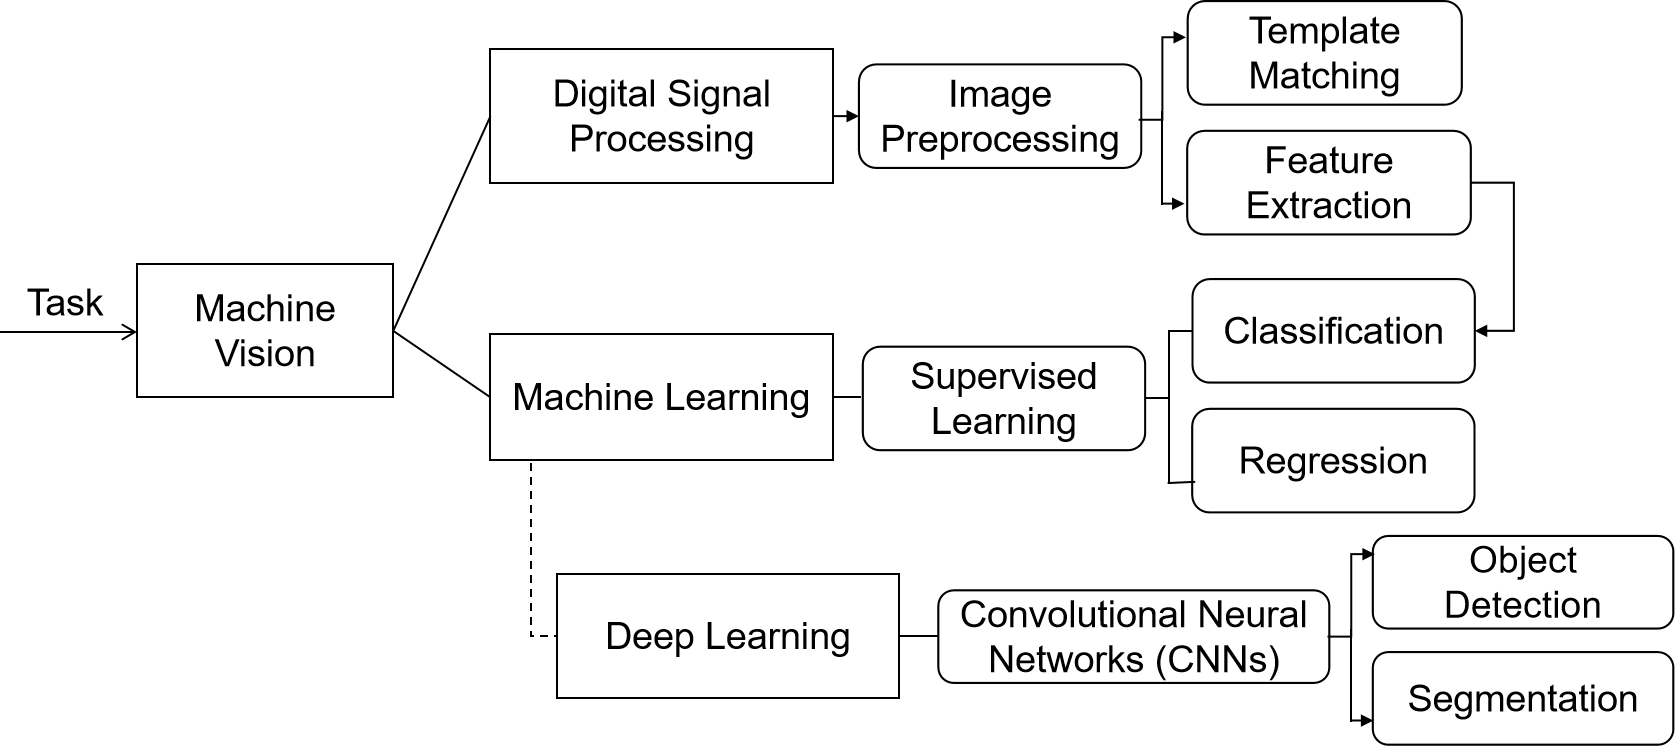
\includegraphics[width=1\textwidth]{Figures/Methodology Overview.png}
  \caption{Methodology Overview}
  \label{fig:1}
\end{figure}

\section{Digital Signal Processing}

Digital Signal processing techniques can be applied to process digital images. A digital image is a two-dimensional matrix of pixel points, each with certain brightness and color information. By using DSP techniques, we can analyze these pixel points to extract useful information. Such process is called digital image processing. It mainly includes the following aspects: Image preprocessing, feature extraction and template matching.

\subsection{Image Preprocessing}

Due to the complexity of the acquisition environment and lighting, the quality of the image can be greatly disturbed, which in turn affects the accuracy of recognition. Therefore, before the image is recognized, the necessary preprocessing operations need to be performed. Basic preprocessing operations include graying, binarization, smoothing, enhancing, scaling, rotating and edge detection.

\textbf{Graying} is the process of changing the image to grayscale, while \textbf{binarization} changes the grayscale image into a grayscale image with values of 0 and 255. These two operations reduce the amount of data in the image and simplifies the image processing. \textbf{Smoothing} removes detailed information from images to reduce noise and image distortion, where median filter is a commonly used technique. \textbf{Enhancing} aims to improve the contrast, brightness, and detail of images, making them sharper and easier to see. Histogram Equalization is the state-of-art. \textbf{Scaling} and \textbf{rotating}, as their names indicate, change the size, direction, angle of the image for better follow-up processing and analysis. 

\textbf{Edges} are very important features of an image in machine vision. This is because edges represent the demarcation line between different regions, and such division is crucial for segmentation and object recognition. \textbf{Edge detection} is the operation to detect such edges in the preprocessing stage. Canny algorithm \cite{canny_computational_1986} is a widely used gradient-based edge detection algorithm which can accurately detect edges in the image with good noise immunity and efficient performance. Figure \ref{fig:2} shows the effect of aforementioned preprocessing operations. 

\begin{figure}[h]
  \centering
  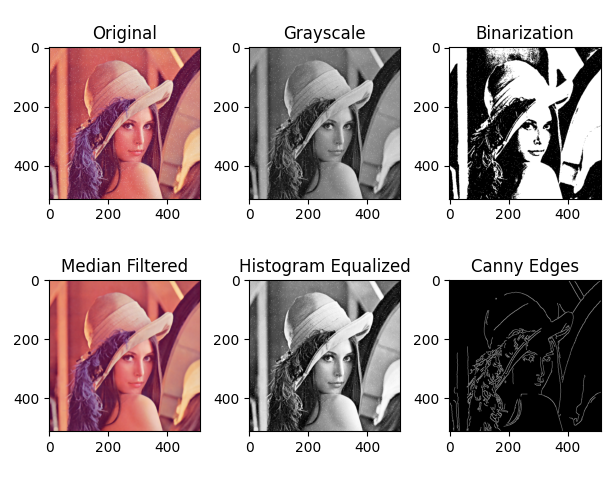
\includegraphics[width=0.7\textwidth]{Figures/Image Preprocessing.png}
  \caption{Effect of multiple preprocessing operations}
  \label{fig:2}
\end{figure}

\subsection{Template Matching}

\textbf{Template matching} refers to finding the part of the test image that is similar to the template image by comparing between the template image and the test image, which is achieved by calculating the similarity between the template image and the target in the test image, and can quickly locate the predefined target in the test image. A template can be an example, an instance; esp. a typical model or a representative instance  \cite{brunelli2009template}.

Template matching is very similar to the principle of convolution, the template slides on the original image from the origin, calculates the degree of difference between the template and the place where the image is covered by the template, then the result of each calculation is put into a matrix and output as the result. After that maximum value in the similarity matrix is found, and this will give a position at which the input image matches the template image to the highest degree. That position is then be used to position the area which matches the template. Figure \ref{fig:3} shows an example of template matching.

Template matching is a simple and efficient way to detect the target object. Compared to 
machine learning techniques, template matching does not require a large amount of training data and can therefore be used when the amount of data is limited. However, such method is sensitive to image transformations, and even slight environment changes would cause the failure, letting alone tackling the problem of occlusion. In order to improve the stability and accuracy of the algorithm, techniques like scale and rotation invariant feature detection are used to extract features from the image.

\begin{figure}[h]
  \centering
  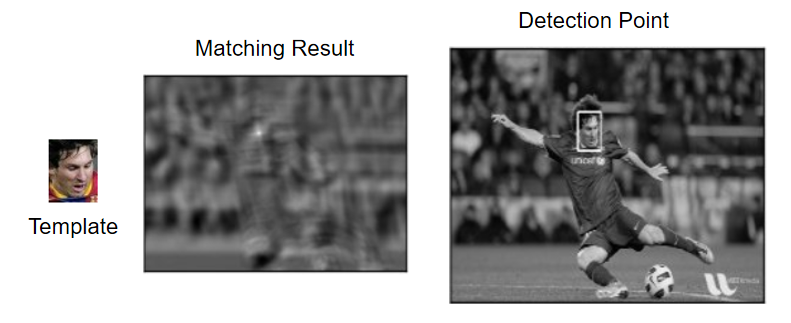
\includegraphics[width=1\textwidth]{Figures/Template_Matching.png}
  \caption{An example of template matching in OpenCV} \cite{opencv}
  \label{fig:3}
  
\end{figure}


\subsection{Feature Extraction}

Feature extraction is the basis of object recognition, which can extract important information from images like feature points. These feature points can be kept constant at different scales and angles, thus improving the accuracy of object recognition and classification. Several common feature extraction techniques are described below:

\textbf{Harris corner detector} \cite{harris1988combined}, as the name infers, is used to extract corner feature points by calculating the difference in gray value between a pixel point in the image and its surrounding pixel points. 

\textbf{scale-invariant feature transform (SIFT)} \cite{lowe1999object} transforms an image into a large collection of feature vectors, each of which is invariant to image translation, scaling, and rotation, partially invariant to illumination changes, and robust to local geometric distortion. Several improvements have been made in its improved algorithm \textbf{Speeded-up robust features (SURF)} \cite{bay2008speeded}.

\textbf{Oriented FAST and rotated BRIEF (ORB)} \cite{rublee2011orb} is a faster, more robust local feature detector modified from SIFT and SURF to detect features points in images and generate descriptors. However, it is less robust to different lighting conditions and occlusion.

After feature descriptors are extracted, they are used as input to train the classifier which is then used for classification or object detection. Related machine learning terms will be explained in the next section.

\section{Machine Learning}

\textbf{Machine learning} is a sub-field of artificial intelligence that is concerned with building useful algorithms rely on a collection of examples, no matter naturally or artificially generated \cite{burkov2019hundred}.

\subsection{Supervised Learning}

\textbf{Supervised learning} is one of the categories and the most common learning method of machine learning. The aim of supervised learning is to build a model that makes predictions based on evidence in the presence of uncertainty. A supervised learning algorithm takes a pre-labelled input data and known responses to the data (output) and trains a model to generate reasonable predictions for the response to new data. Such a predictive model can be based on two techniques: classification and regression, predicting discrete and continuous responses respectively. Most image-focused pattern-recognition tasks usually depend on classification using supervised learning.

\subsection{Classification}

\textbf{Classification} is the task which automatically assigning a discrete label to an unlabeled example, for example, assigning a given email to the "spam" or "non-spam" class. \cite{burkov2019hundred}

A classification problem in machine learning is typically addressed through the use of a classification learning algorithm. These algorithms take a set of labeled examples as input and generate a model that can be used to predict the label of a new, unlabeled example. The output of the model can be either a directly assigned label, or a numerical value that can be interpreted by an analyst to deduce the label.

\textbf{Support Vector Machine (SVM)} is a type of classifier commonly used to tackle two-group classification problems. The machine conceptually implements the following idea: input vectors are non-linearly mapped to a very high-dimension feature space \cite{cortes1995support}. In machine learning, the boundary separating the examples of different classes is called the decision boundary \cite{burkov2019hundred}. The algorithm aims to construct a maximally spaced hyperplane during the training so that the decision boundary has the maximum margin between the closest samples. 

The evaluation of the classification result can be done by a \textbf{confusion matrix}, which can classify the test data into four categories: true positives (TP) , false positives (FP), true negatives (TN) and false negatives (FN). Correct Classification Rate (CCR) , a common assessment metric of classification models, can then be calculated as follow:

$$
   \text{CCR} = \frac{\text{TN} + \text{TP}}{\text{FN} + \text{FP} + \text{TP} + \text{TN}}
$$

An example is shown in figure \ref{fig:4}. As can be seen, the decision boundary L1 is set too close to the training samples, while L2 obtained by SVM algorithm maintains the largest margin. Two boundaries may make different predictions to the test sample marked in the figure, and these results are evaluated differently in the confusion matrix (FN for L1 and TP for L2). This can show how L2 may obtain a better CCR as similar test samples increases.

\begin{figure}[h]
  \centering
  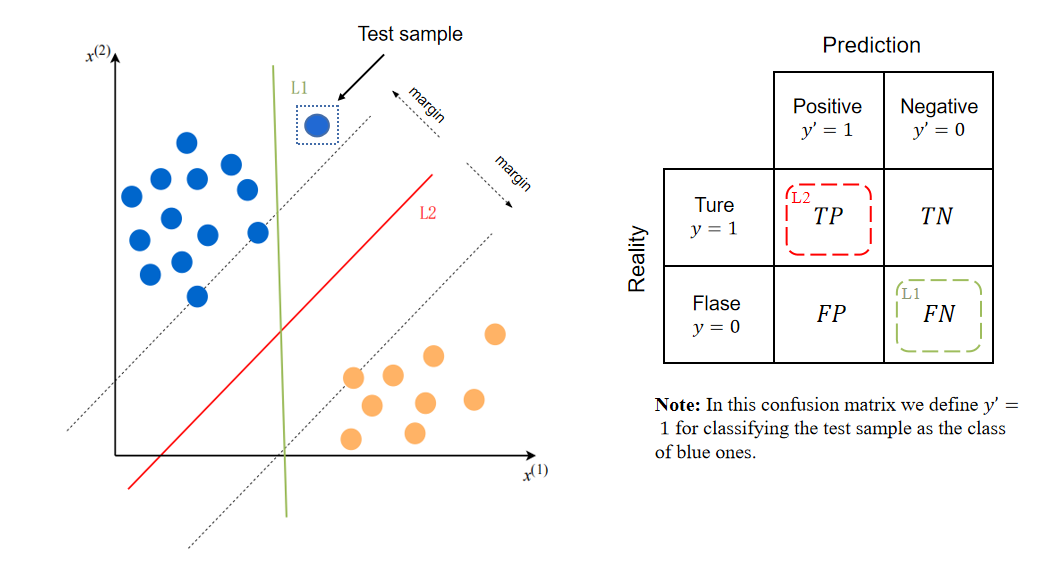
\includegraphics[width=0.8\textwidth]{Figures/SVM and confusion matrix.png}
  \caption{An example of SVM decision boundary (left) and the confusion matrix (right). L1 fails to classify the marked test sample correctly}
\cite{burkov2019hundred}
  \label{fig:4}
\end{figure}

\subsection{Regression}

\textbf{Regression} is the task of predicting a real-valued label (often called a target) given an unlabeled example, for example, estimating stock price \cite{burkov2019hundred}.

In supervised learning, a regression problem chooses a regression algorithm to take a collection of labeled examples as inputs and produces a model that can take an unlabeled example as input and output a target. The relation between predicted output and input can be expressed as $ y' = f (x) $. Based on the function, a regression problem can be classified as linear regression, polynomial regression, etc. During the training of a regression model, \textbf{loss function} is used to evaluate the performance by calculating the error between predicted and true values. Mean Squared Error (MSE) is a common loss function, which can be calculated by $ MSE = \frac{1}{n}\sum_{i=1}^{n}(y_i - \hat{y}_i)^2$. The smaller the MSE, the better the performance of the model will be. Figure \ref{fig:5} depicts an example of a linear regression model and the corresponding MSE.

\begin{figure}[h]
  \centering
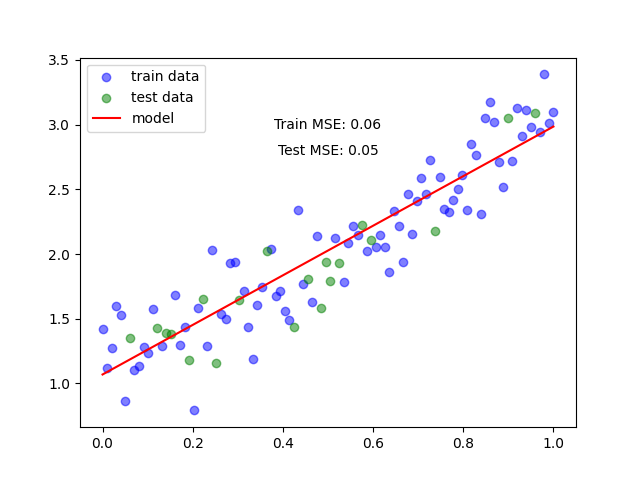
\includegraphics[width=0.5\textwidth]{Figures/Linear Regression.png}
  \caption{An example of a linear regression model}
  \label{fig:5}
\end{figure}

In order to minimize the loss function of the model, \textbf{gradient descent algorithm} is used to obtain the best model parameters. Gradient descent algorithm is an iterative optimization algorithm that reduces the value of the loss function by calculating the partial derivatives (gradient) of the loss function with respect to the model parameters and updating the model parameters along the negative gradient direction. The algorithm is used to continuously update the model parameters, and the optimal regression model can be gradually fitted to minimize the error between the prediction result and the true value.

Traditional machine learning classification and regression methods can largely improve the adaptability to different scenarios and tasks compared to the traditional digital signal processing. However, their generalization capabilities are still insufficient, while a large number of manual rules still need to be designed for feature extraction and dealing with occlusion.


\section{Artificial Neural Networks (ANNs) and Deep Learning}

\textbf{Artificial neural networks (ANNs)} is a very useful tool in supervised learning and is the foundation of deep learning. ANNs are computational processing systems of which are heavily inspired by way biological nervous systems (such as the human brain) operate. ANNs are mainly comprised of a high number of interconnected computational nodes, which we name as neurons. These neurons work distributively to collectively learn from the input in order to optimise its final output.

Figure \ref{fig:6} shows the architecture of a simple ANN and how a neuron processes its input. For every neuron, it calculates the sum of every input, which is the output of each neuron in the previous layer, with \textbf{weights} set to each input to measure its influence on the result. A \textbf{bias} is also set to adjust the intermediate result for \textbf{activation} afterward. The goal of activation is to add non-linear features into the output of a neuron, which helps neural networks discover and learn complex patterns, and to normalize such output to be an input of the next layer. Rectified Linear Unit (ReLU) is one of the commonly used activation functions, which simply turns all negative output values to 0.

An ANN is generally composed of three types of layers. The input layer loads inputs in the form of a multidimensional vector to the input layer, and distribute them to the hidden layer. The hidden layer will then make decisions from the previous layer and weigh up how a stochastic change within itself detriments or improves the final output, and this is referred to as the process of learning. Having multiple hidden layers stacked upon each-other is commonly called deep learning \cite{oshea_introduction_2015}.

\begin{figure}[h]
  \centering
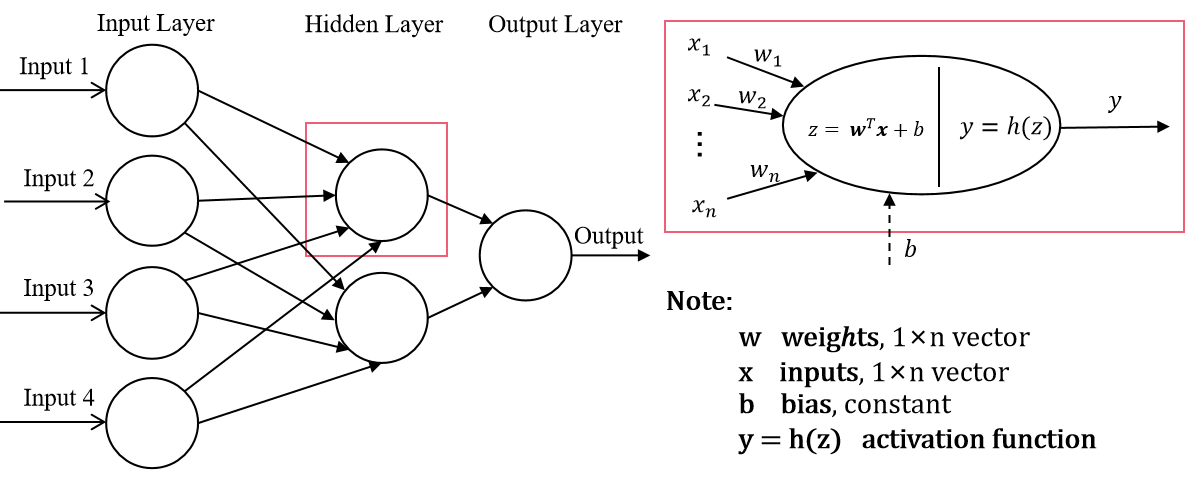
\includegraphics[width=1\textwidth]{Figures/ANN-architecture.png}
  \caption{The architecture of a simple ANN network}
  \label{fig:6}
\end{figure}

One of the largest limitations of traditional forms of ANNs is that when computing image data, they tend to struggle with the computational complexity. This is because each neuron in fully-connected layers needs to be connected to all neurons in the previous layer, and this require a lot of computation to deal with the huge number of weights each neuron provides for every single pixel. Besides, even if the computing power is unlimited, the complexity will cause another problem: overfitting, which occurs when a model is trained too well on a particular data set, to the extent that it starts to fit the noise or random fluctuations in the data rather than the underlying patterns or trends, resulting in poor performance on new, unseen data. In order to reduce the complexity of ANNs, \textbf{Convolutional Neural Networks (CNNs)} is introduced. 

\subsection{Convolutional Neural Networks (CNNs)}

CNNs are analogous to traditional ANNs in that they are comprised of neurons that self-optimise through learning. The notable differences between two networks are their architectures, which makes CNNs more capable in the field of pattern recognition within images.

Figure \ref{fig:6} depicts the architecture of a general CNN. The basic functionality of this example CNN can be broken down into three key areas: convolutional layers, pooling layers and fully-connected layers.

\begin{figure}[h]
  \centering
  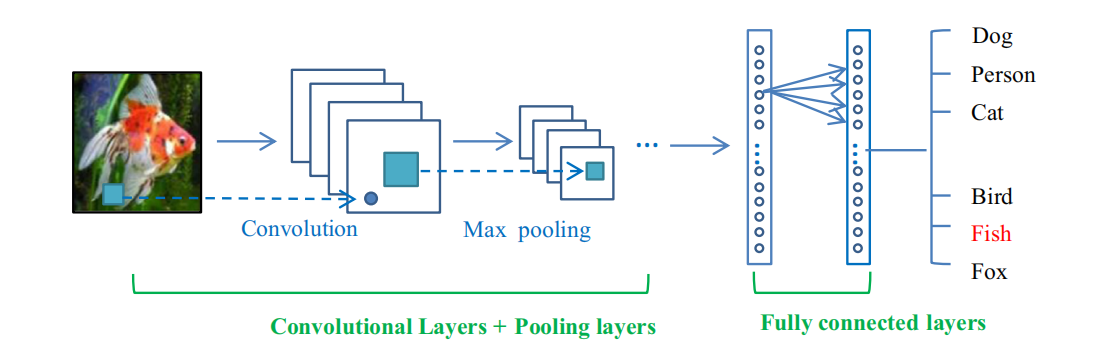
\includegraphics[width=1\textwidth]{Figures/CNN-architecture.png}
  \caption{The pipeline of the general CNN architecture \cite{guo_deep_2016}}
  \label{fig:6}
\end{figure}

As can be implied from the name, \textbf{convolutional layers} play a vital role in how CNNs operate. Its main task is to extract features from the original input image by convolution operations. The output of the convolution layer can be used as the input of the next layer. 

Feature extraction in the convolutional layers is realized by several learnable convolution \textbf{kernels}, which are used to convolve the input image to produce an output feature map. In a CNN, each neuron of the convolutional layer uses a kernel to process the input pixels adjacent to it. Every kernel can serve as a filter to extract one specific feature of the input image like edges, corners, etc. Since such filters can be applied to any part of the input image and each type of filters is sharing the same parameters, the number of parameters we required is dramatically decreased. This important feature is called \textbf{parameter sharing}, which can reduce the risk of overfitting and improving the generalization ability of the model. 

During the convolution operation, a kernel is used to slide over the input image, performing one convolution operation at a time, to produce the output feature map. As the input is glided through, the scalar product is calculated for each value in that kernel. Then activation function will be applied, and every kernel will obtain a corresponding activation map, of which will be stacked along the depth dimension to form the full output volume from the convolutional layer.

There are three hyperparameters that control the size of the output volume of the convolutional layer: depth, stride and zero-padding. \textbf{Depth} refers to the number of convolutional kernels in the convolutional layer. \textbf{Stride} is the distance that the filter moves along the input each time. \textbf{Zero-padding} is the simple process of padding the border of the input by setting it zero.

A \textbf{pooling layer} is usually attached after convolutional layers. It contains pooling operations used to reduce the size of the convolutional layer outputs, thereby reducing the model complexity and computing power required. Pooling operations can also improve the robustness and generalization of the model to reduce the risk of overfitting. The most commonly used pooling function is max pooling and average pooling, which take the maximum value in the pooling window as output.

Following several convolutional and pooling layers, \textbf{fully-connected layers} perform the high-level reasoning in CNNs. As the name implies, every neuron in fully connected layer has full connections to all activation in the previous layer. Their activation can then be calculated with a matrix multiplication with a bias offset. The fully connected layer eventually converts the 2D feature map into a 1D vector. The vectors derived can either be fed into a certain number of classifications or can be considered as feature vectors for further processing \cite{voulodimos_deep_2018}. 

The input data is processed through convolutional layers, pooling layers, etc., and finally the prediction result of the model is obtained in the output layer. Such process is defined as forward propagation. However, the predicted value may have deviation from the real one to some extent. In order to diminish such deviation, we need use loss functions to calculate the deviation and updates each parameter by \textbf{back propagation} to minimize the loss. Similar to the process introduced in the regression model training, gradient descent algorithm is also used in back propagation for calculating new weights in that procedure.

\subsection{Object detection}

Object detection aims to automatically identify and localize a specific class of objects from an image or video. The target objects are marked given their locations via \textbf{bounding boxes}. In recent years, the development of deep learning has made significant progress in object detection. Deep learning-based object detection methods include two main types: single-stage detection and two-stage detection.

\textbf{Single-stage detection} requires only one neural network model, performing forward propagation only once to complete the object detection. Therefore, it is an efficient method but with sometimes lower precision. \textbf{You Only Look Once (YOLO)} is a representative single-stage detection algorithm. Its main idea is to divide the feature map obtained from the output of CNN into multiple grids, with each grid predicting a fixed number of bounding boxes and their corresponding object class probabilities. Then, category probabilities and position information of each bounding box are adjusted to obtain the final prediction box. Finally, the Non-Maximum Suppression (NMS) algorithm is applied to remove redundant bounding boxes and obtain the detection results \cite{redmon2016you}. Besides the YOLO series, Single Shot MultiBox Detector (SSD), RetinaNet are another single-stage detection algorithms.

\textbf{Two-stage detection} can offer better accuracy. It involves two steps: proposal generation and detection. In the first stage, a region proposal network generates potential bounding boxes, and in the second stage, features of the proposed regions are extracted and used to classify and refine the boxes. \textbf{Faster R-CNN} and \textbf{Mask R-CNN} are two of the most popular two-stage detection algorithms.

\subsection{Segmentation}

Unlike object detection, segmentation requires classification of each pixel in the image, rather than localizing and classifying only the boundaries of the object. Based on different 
segmentation results, it can be categorized into three types: semantic segmentation, instance segmentation and panoptic segmentation.

\textbf{Semantic segmentation} is an approach detecting, for every pixel, belonging class of the object \cite{guo2019degraded}. For example, all cars in an image are segmented as one object and background as another object. There will be distinctions between two different cars in reality. \textbf{U-Net}, named by its U-shape architecture \cite{ronneberger2015u}, is one of the stage-of-art based on CNN to process semantic segmentation.

\textbf{Instance segmentation} aims to identify the every pixel's belonging of object. It detects each distinct object of interest in the figure. For instance, every car in a figure is segmented as an individual object. \textbf{Mask R-CNN}, which is mentioned above as an object detection algorithm, can also be used in instance segmentation task. 

\textbf{Panoptic segmentation} combines the feature of semantic and instance segmentation. It can identify the belonging class of each pixels, meanwhile distinguishing them based on different instance. However, to realize both features requires processing a large number of object instances and backgrounds simultaneously, and thus requires more resources. \textbf{Panoptic FPN} and \textbf{BlendMask} can be some of the commonly used algorithms.

In Figure \ref{fig:7}, we can see an example of how object detection, semantic segmentation, and instance segmentation can be applied to the same image. The selection of the appropriate method depends on the specific task requirements and scenarios, which will be thoroughly discussed in the following chapter.
\begin{figure}[h]
  \centering
  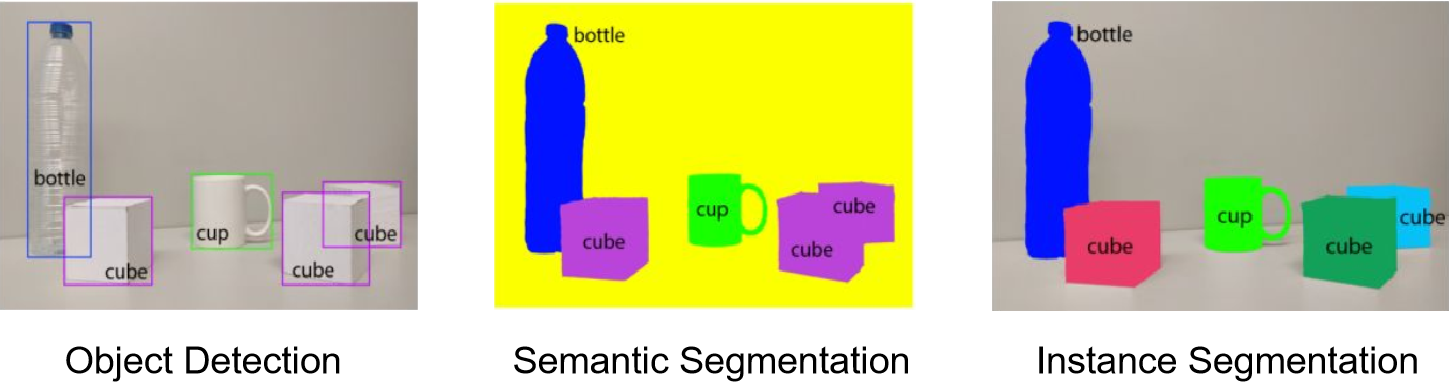
\includegraphics[width=1\textwidth]{Figures/Object detection and segmentation.png}
  \caption{An example of object detection and segmentation}
  \cite{nitish_2017}
  \label{fig:7}
\end{figure} 
\chapter{Concept}\chaplabel{3}

This chapter aims to identify a promising approach to address the task. A thorough analysis of the challenges associated with the task is conducted first. This analysis serves as a foundation for comparing and contrasting different methods and algorithms to determine the most effective approach.

\section{Task Challenges}

This study is confined to a particular building on the THL campus, and concentrates on a single facade. As a result, the roller shutters installed on this particular building are relatively homogeneous in terms of their features, such as texture, brands, and colors. Additionally, the images used for analysis are static, and do not require real-time processing. Despite these factors, the realization of the proposed detection method may face several challenges. Three main challenges are identified and discussed in the following sections.

\subsection{Round-the-clock detection}

Detecting objects reliably under different weather conditions and at different times of day poses a challenge. Changes in light intensity and color temperature can significantly affect the appearance features of roller shutters, while camera's performance may also degrade due to factors such as lighting and noise, thereby affecting the image quality. Figure \ref{fig:8} depicts how the image of the same window would differ under various conditions. 

\begin{figure}[h]
  \centering
  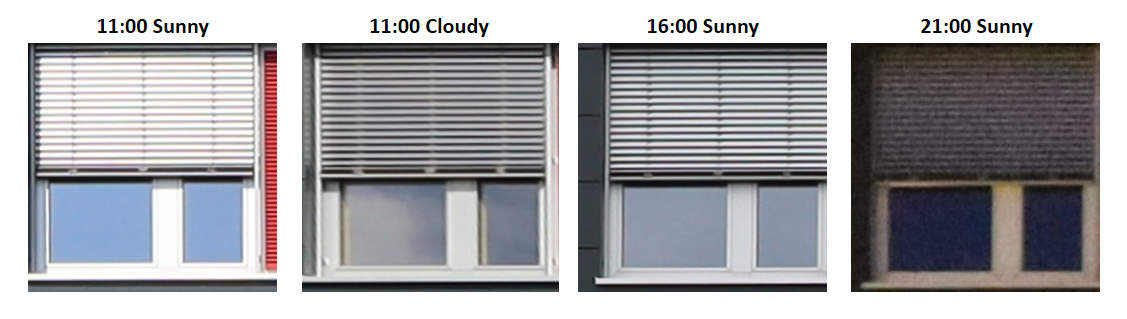
\includegraphics[width=1\textwidth]{Figures/round-the-clock.png}
  \caption{Images of the same window taken at different time or under different weather conditions}
  \label{fig:8}  
\end{figure}

\subsection{Impact of occlusion}

Occlusion is considered a existing and challenging issue in machine vision applications that can significantly hinder feature extraction and classification when the target is obscured. The problem is further exacerbated in the current study, where not only the roller shutter need to be detected, but its degree of closure must also be calculated. Figure \ref{fig:9} describes examples of occlusion scenarios in this task. Addressing this challenge requires a highly demanding solution to mitigate the impact of occlusion.

\begin{figure}[h]
  \centering
  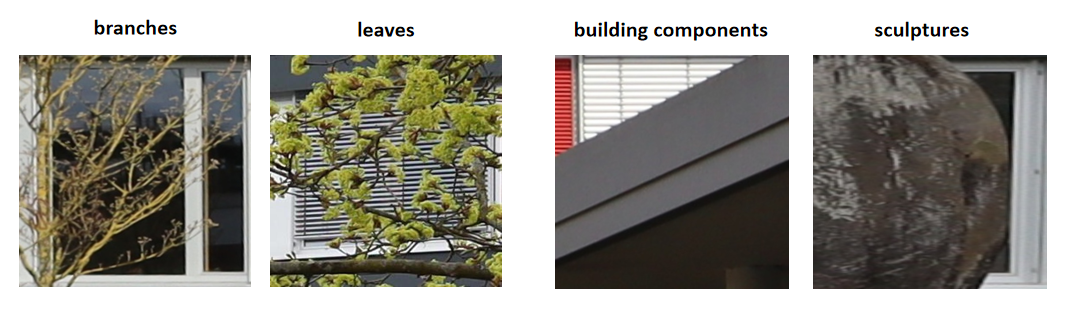
\includegraphics[width=1\textwidth]{Figures/occlusion examples.png}
  \caption{Images of various occlusion scenarios}
  \label{fig:9}  
\end{figure}

\subsection{Measurement of the Degree of Closure (DoC)}

In order to accurately determine the percentage of how much a roller shutter is lowered (In this bachelor thesis, DoC is used to represent such percentage) , a reliable and consistent measurement method that can be applied to all situations is necessary. While the length and area of a window remain fixed in the real world, the shape of the window in the 2D world of digital photography can be affected by the camera angle, making it challenging to obtain clear and upright images for accurate measurements. Additionally, distinguishing the boundary between the window and the roller shutter may also pose difficulties.

\section{Evaluation of Methods}

In chapter 2, three promising methods were introduced, which are:

\begin{enumerate}
  \item traditional digital signal processing techniques like template matching
  \item traditional machine learning with classification and regression
  \item deep learning with object detection and segmentation
\end{enumerate}

Based on their performance for addressing the challenges mentioned above, one method will be selected for use in this study. This section presents an analysis of the strengths and limitations of each method. In order to ensure simplicity throughout this section, this bachelor thesis employs \textbf{DSP Method, TML Method} and \textbf{DL Method}, respectively, to represent these methods. Table \ref{tab:1} provides an overview of the performance of the three methods in addressing the challenges posed by the task, which would be explained in the following paragraphs.

\begin{table}
  \centering
  \caption{Evaluation of Three Methods}
  \label{tab:1}
  \begin{tabular}{cccc}
    \toprule
    Methods & Round-the-clock Detection & Occlusion & Measurement \\
    \midrule
    DSP Method &  + & - & + \\
    TML Method & ++ & + & + \\
    DL Method & +++ & ++ & ++ \\
    \bottomrule
  \end{tabular}
  \vspace{0.8em}
  \begin{tablenotes}
    \item \textbf{Note:} The more plus signs (+) indicate better performance, while the minus sign (-) indicates the method is not suitable for addressing the challenge.
    
  \end{tablenotes}
\end{table}

The first challenge is round-the-clock detection, for which the DL method performs the best. DSP Method can be a fast and simple solution, but it requires several preprocessing steps to reduce the impact of lighting or noise. However, these steps should be designed carefully while adaptive processing steps may hinder the accuracy of detection to a great extent. The TML method has the advantage of being able to classify or regress new and unknown patterns or scenarios by learning the statistical patterns of the data, thus having stronger generalization ability. However, it still requires manual feature engineering, which demands specific knowledge and experience. On the other hand, DL method may require some time to train the model, but it can overcome the limitations of the other two methods. By learning large amounts of data, DL can automatically extract features and better generalize to new data. Since the speed of detection and training time are not the primary requirements of this study, the DL method is considered the most appropriate for addressing round-the-clock detection issues.

The second challenge is occlusion. DL method still performs best in tackling this issue. DSP Method like template matching relies on comparing the raw pixel values of the input image to a pre-defined template, which is not robust to changes in the appearance of the object due to occlusion. The TML method can improve the robustness of the model by selecting features that are insensitive to occlusion, and the classifier design can use a combination of multiple classifiers to mitigate the effects of occlusion. However, for different occlusion cases, the features need to be manually selected and designed again, which makes the implementation and adjustment of the algorithm more cumbersome. The DL method provides a better solution with the help of data augmentation in the training process, and can automatically learn feature representations in images, enabling them to recognize objects even when they are partially occluded. DL models can also incorporate multiple scales and viewpoints of the object to improve recognition accuracy.

In terms of measuring the DoC, the shape of the roller shutter is rectangular, which matches the shape of a bounding box. Therefore, using bounding boxes as a representation is considered appropriate for this study. Although all three methods can provide bounding boxes to locate the target, the DL method can provide more detailed and accurate bounding boxes, as well as other information such as the class and confidence level of the target. This additional information enables more comprehensive and precise object detection and recognition, using techniques such as Non-Maximum Suppression (NMS), which outputs only the bounding boxes with the highest confidence level in a certain region. If a pixel-level measurement of DoC is required, a deep learning segmentation task can generate a mask of the roller shutters to improve the measurement accuracy.

Overall, the superior performance of the DL method, which surpasses the other two methods in every aspect, makes it the preferred approach for this bachelor thesis.

\section{Evaluation of Algorithms}

In order to select the most efficient algorithm for the current task, it is crucial to evaluate the candidate deep learning algorithms. While both object detection and segmentation algorithms can achieve recognition, this bachelor thesis will only focus on algorithms primarily designed for object detection. This is because although segmentation can provide precise classification of every single pixel, it requires far more training to achieve the same level of accuracy as object detection. On the other hand, as is mentioned above, the use of rectangular bounding box would be enough for measurement. 

In the previous chapter, several one-stage and two-stage object detection algorithms were mentioned. This bachelor thesis includes R-CNN series, EfficientDet, YOLO series, RetinaNet, and SSD series as candidates for evaluation. To analyze the performance of these algorithms, two metrics were considered: Mean Average Precision (mAP) and Frames Per Second (FPS). While real-time detection was not a requirement for the task, higher FPS could indicate faster processing times when handling a large number of static images, and was therefore taken into consideration.

This bachelor's thesis compiled the test results of each algorithm's most complex model (which maximize the mAP at the cost of FPS) on the COCO dataset (test-dev2017), as shown in Table \ref{tab:2}. It can be seen that the later YOLO series achieved a generally higher mAP and faster detection speeds compared to the other algorithms. Among the YOLO series, YOLOv5 may be not the latest version of YOLO series, but it remains one of the state-of-art algorithms in the field of object detection and more researches are based on it than any other YOLO's later version. Therefore, this bachelor thesis chooses YOLOv5-v6.0 as the proposed algorithm to address the detection of roller shutter status.

\begin{table}
  \centering
  \caption{Performance on COCO Dataset}
  \label{tab:2}
  \begin{tabular}{cccccc}
    \toprule
    Algorithms & Proposal & Backbone & Size & FPS & mAP (\%) \\
    \midrule
    \midrule
    Faster R-CNN \cite{wang2019region} & 01/2016 & ResNet-50 & - & 9.4 & 59.2 \\
    R-FCN \cite{redmon} & 03/2016 & ResNet-101 & - & 12 & 51.9 \\
    FPN FRCN \cite{redmon} & 10/2017 & ResNet-101 & - & 6 & 59.1 \\
    \midrule
    RetinaNet \cite{lin2017focal} & 06/2018 & ResNet-101 & 800 & 5.1 & 57.5 \\
    \midrule
    EfficientDet-D3 \cite{tan2020efficientdet} & 03/2020 & Efficient-B3 & 896 & 23.8 & 65.0\\
    \midrule
    SSD \cite{liu2016ssd} & 12/2016 & VGG-16 & 512 & 22 & 48.5 \\
    SSD \cite{redmon} & 12/2016 & ResNet-101 & 513 & 8 & 50.4 \\
    DSSD \cite{redmon} & 07/2017 & ResNet-101 & 513 & 6 & 53.3 \\
    \midrule
    YOLOv3-SPP \cite{redmon2018yolov3} & 04/2018 & Darknet-53 & 608 & 20 & 60.6 \\
    YOLOv4 \cite{bochkovskiy2020yolov4} & 04/2020 & CSPDarknet-53 & 608 & 23 & 65.7 \\
    YOLOv5x \cite{ultralytics} & 05/2020 & CSPDarknet-53 & 640 & - & 68.9 \\
    YOLOv5x6 \cite{ultralytics} & 05/2020 & CSPDarknet-53 & 1280 & - & 72.7 \\
    \bottomrule
  \end{tabular}
  \vspace{0.8em}
  \begin{tablenotes}
    \item \textbf{Note:}  (-) indicates that the corresponding metrics were not found.
    
  \end{tablenotes}
\end{table}

\section{Addressing Challenges Using Bounding Boxes}

Now that object detection algorithm YOLOv5 is selected for this task, how it can solve the existing challenges need to be discussed before moving on to the implementation part. One of the main features of YOLOv5 and other object detection algorithm is using bounding boxes to localize the object. Although the performance of an algorithm can be decided by its architecture to a large extent, the ability to tackle specific challenges can be improved if the bounding boxes are used wisely and certain rules are set.

As the round-the-clock detection can be well realized through existing YOLOv5 network architecture and feature extraction strategies, this section focuses mainly on the newly proposed solutions for addressing occlusion and measurement of DoC in roller shutter detection.

\subsection{Solution for heavy occlusion}

Unlike the common goal of object detection algorithms, which is to recognize objects despite all kinds of occlusion, the goal of this task is not only to recognize but also to provide precise measurements. Therefore, we do not want the model to sacrifice the accuracy of measurements by predicting the possible area of the entire roller shutter in the presence of heavy occlusion. To address this, a balance is defined to split occlusion scenarios into two categories: \textbf{Mild occlusion}, which the model should be robust enough to “see through”, such as branches, leaves; \textbf{Heavy occlusion}, which should be exclude by the model, such as building components, sculptures, regardless of whether the part obscured is part of roller shutters. For heavy occlusion scenarios, this subsection will explain how a decision tree can be applied to tackle them.

To achieve this, the status of roller shutters are set as open, closed or blocked. This gives rise to another problem when we defining object classes. If we set shutter as the only object class, there will be only two different results based on whether roller shutters are detected or not. To be more specific, if roller shutter is not detected in the image, the status could either be open or blocked, which we cannot tell from each other based on the detection results. Therefore, this bachelor thesis add another object class to detect window glass, which can help determine the status.

As shown in Figure \ref{fig:10}, ten scenarios are used to simulate the roller shutter status in reality. In some scenarios, although strong occlusion exists in the images, it has no influence on the determination of roller shutter status. This is because we only need to find out the demarcation between roller shutters and glass to judge the DoC. Therefore, as long as such demarcation is clear, any occlusion would not be considered affecting the detection result. This also give rise to another method to calculate DoC, which will introduced later in this section.

\begin{figure}[h]
  \centering
 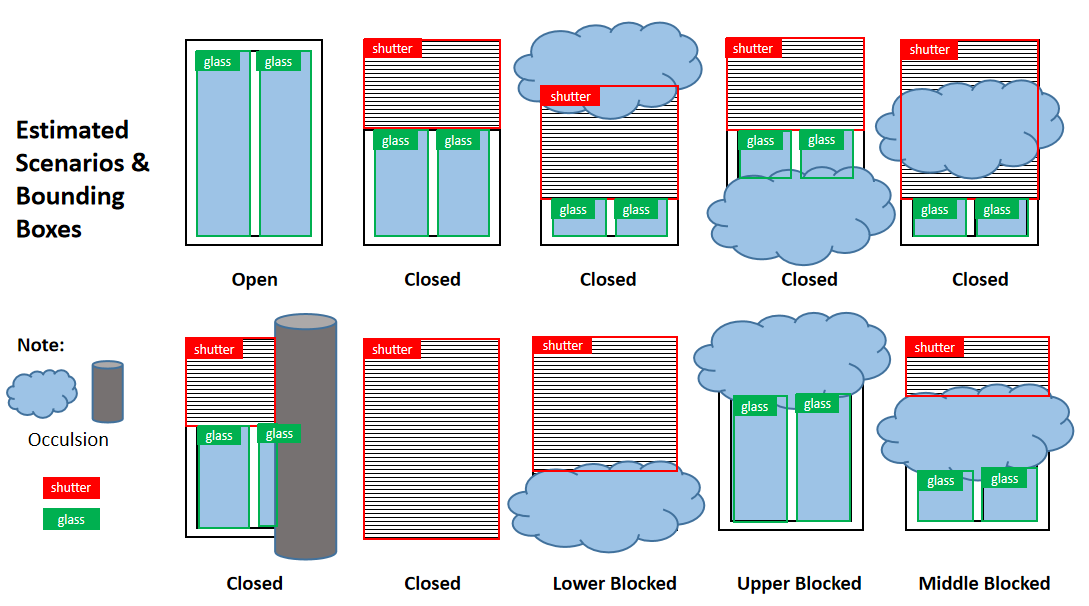
\includegraphics[width=1\textwidth]{Figures/Estimate BBs.png}
  \caption{Estimated Scenarios and Bounding Boxes with Two Object Classes "Shutter" and "Glass"
}
  \label{fig:10}
\end{figure}


\begin{figure}[h]
  \centering
 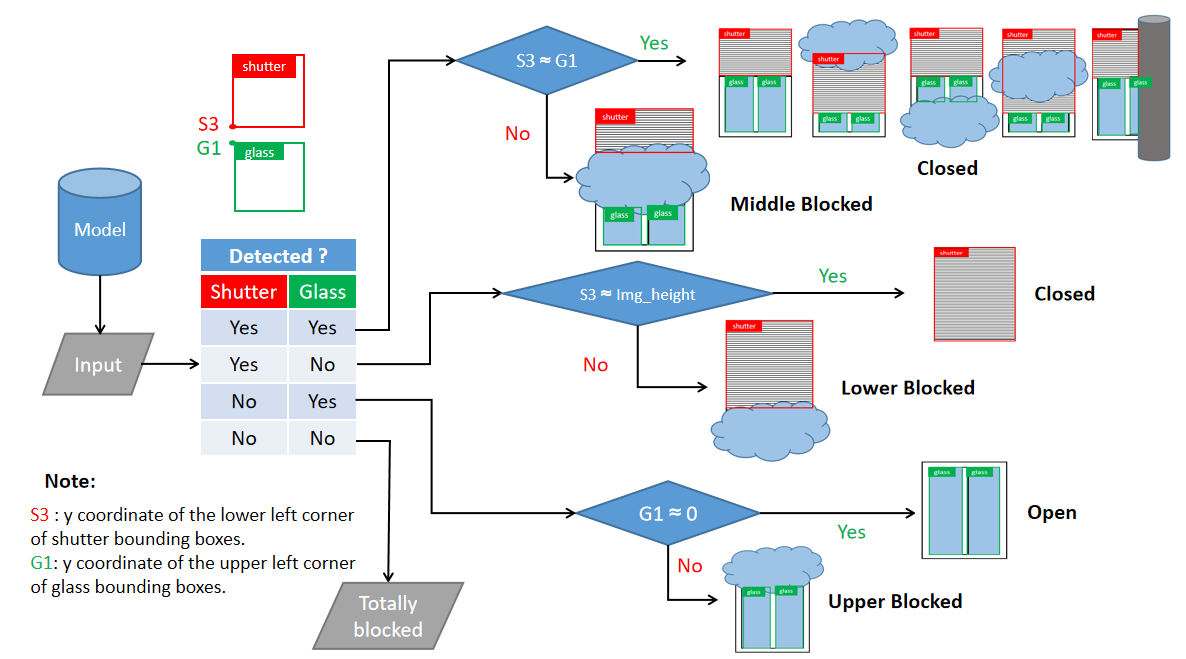
\includegraphics[width=1\textwidth]{Figures/Decision Tree.png}
  \caption{A Decision Tree to Determine The Roller Shutter Status
}
  \label{fig:11}
\end{figure}

To distinguish these scenarios by status, a decision tree is designed as figure \ref{fig:11} depicts, those scenarios can be split by simple logic comparing a few parameters of the bounding boxes. To be specific, \textbf{S3} and \textbf{G1}, which represent y coordinates of the lower left corner of shutter bounding boxes and the upper left corner of glass bounding boxes respectively. Those scenarios are split into four branches at first step based on the detection results:

\textbf{(1) Both the roller shutter and glass are detected.} This means the status is either closed or blocked. We need to examine whether the demarcation between the roller shutter and glass is clear by comparing G1 and S3. If G1 is approximately equal to S3, we can determine that the roller shutter status is closed. Otherwise, something is blocking the window in the middle, and the end of the roller shutter could be anywhere above G1 and below S3.

\textbf{(2) Only the roller shutter is detected.} In this case, we cannot tell whether the window glass is fully covered by the roller shutter or partly by occlusion. Therefore, we compare S3 with the height of the window, which is the height of the image in practice (images for detection contain only the window without any background). If S3 is approximately equal to the height of the image, the roller shutter is considered fully closed. If not, it is considered blocked, and the exact DoC cannot be determined.

\textbf{(3) Only the glass is detected.} With the absence of the roller shutter, we cannot simply say that the roller shutter is open. This is because the roller shutter may be covered by occlusion that covers the upper part of the image. To address this problem, we need to check the value of G1. If it approaches 0, which ensures that the upper parts of the image may not be the roller shutter, then we can determine the status as open. Otherwise, we cannot determine whether the area above G1 in the image is glass or roller shutter, which we mark as blocked.

\textbf{(4) Neither the roller shutter nor glass is detected.} This indicates a failure in detection, which could be due to the poor performance of the detection model or the window being completely blocked by occlusion. Assuming that the algorithm works well, we also mark this scenario as blocked.

By using this logic to determine the roller shutter status, the detection model should be robust enough to handle heavy occlusion. However, the logic is not yet clear enough to put into practice because when comparing two parameters, "approximately equal to" cannot be understand by computer. Specific thresholds need to be determined and adjusted during implementation. Also, for mild occlusion, some optimizations have also been made, which are described in the next chapter. 
\subsection{Measurement of DoC}

The most straightforward way to calculate DoC according to its definition is:

$$ DoC = \frac{\text{Area of the Bounding Box}}{\text{Area of Corresponding Window}} \times 100\%
$$

As mentioned in previous evaluation of methods, the measurement of DoC can be achieved using bounding boxes due to their similar shape to roller shutters. However, The area of the bounding box may not express the true area of the Roller shutter. This is because bounding boxes are upright rectangular with their sides either vertical or horizontal. The roller shutter in the image, on the other hand, may not be upright due to shooting angles. Therefore, before detection, the cropped image of each window needed to be set upright to ensure the edge of the roller shutter in the picture is parallel to the edge of the bounding box. In addition, as the width of roller shutter is equal to the width of window and the height of window can be replaced by the height of cropped image in practice, the formula can simplified as 

$$ DoC = \frac{\text{Height of the Bounding Box}}{\text{Height of Image}} \times 100\%
$$

However, the formula may be flawed in certain situations, as discussed in the previous subsection. Using the height of the bounding box may not be appropriate when dealing with occlusion problems, where the bounding box only represents the unobstructed part of the roller shutter. Therefore, as the y coordinate of the bounding box's upper boundary may be 0 in normal cases, the y coordinate of the lower boundary (S3) is used to represent the height of the roller shutter. The final optimized formula is described as: 

$$ DoC = \frac{\text{S3}}{\text{Height of Image}} \times 100\%
$$

Since the height of the image is fixed and depends solely on the input size of the model, there is only one variable in the formula mentioned above. This means that this measurement method may be more resistant to errors. However, the validity of this formula depends on the assumption that each image for detection is only filled with a complete window, without any offset or redundant background in the vertical direction. While this may pose a challenge for localizing windows, the benefits of reducing error rates and minimizing the number of object classes for detection make it a worthwhile trade-off.

\subsection{Fusion}

To obtain accurate results, fusion is another effective method to mitigate the impact of heavy occlusion. In this bachelor thesis, three cameras are set up to capture images of the same building facade from different angles. This allows us to determine the optimal angle that provides the best representation of the roller shutter status and DoC.

As shown in Figure \ref{fig:13}, we considered all 19 possible scenarios using three cameras and estimated the fusion results for both the roller shutter status and DoC. Our estimation was based on three pre-defined rules, as follows:

\begin{enumerate}
\item The status is considered "blocked" only when all camera angles produce "blocked" results.
\item If the final status is "blocked", the DoC range would describe the possible maximum and minimum values. If multiple cameras detect a "blocked" status, the range would be narrowed as much as possible.
\item If "open," "close," or both are detected, the final status is determined by majority rule. If the final status is "closed," the average of the non-zero DoC values would be taken as the final DoC.
\end{enumerate}

\begin{figure}[h]
  \centering
  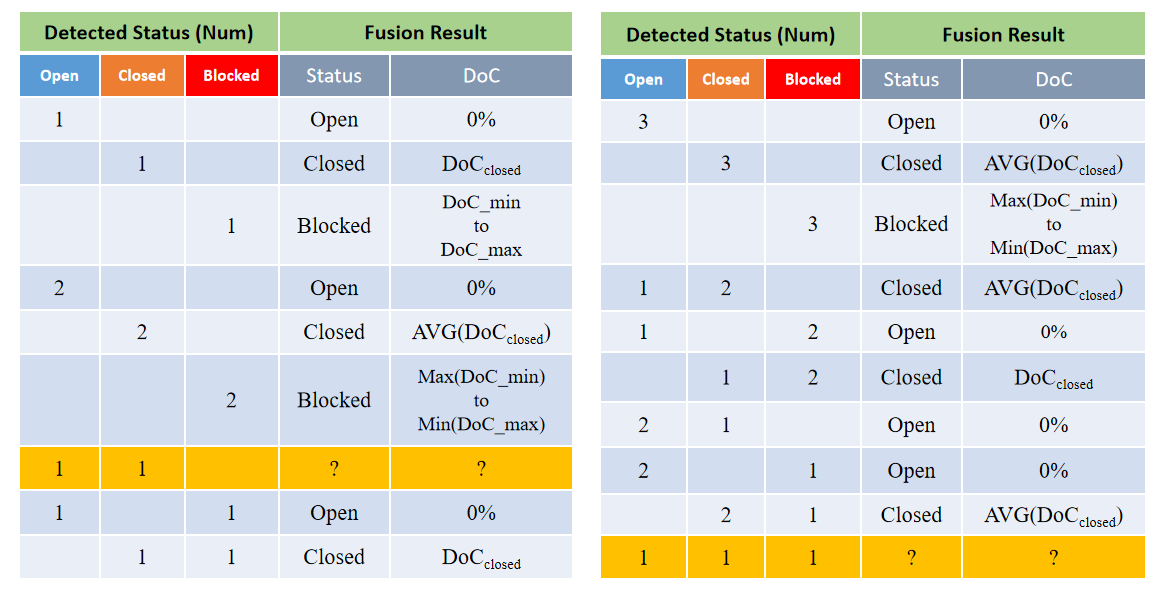
\includegraphics[width=0.9\textwidth]{Figures/Fusion Cases.png}
  \caption{All Detection Cases for up to three cameras and Pre-defined Fusion Results}
  \label{fig:13}  
\end{figure}

The 19 possible scenarios discussed earlier can be summarized and generalized, as shown in Figure \ref{fig:14}, based on the fusion results obtained through the pre-defined rules. However, in situations where the number of "open" and "closed" results are equal, it is difficult to determine the final status of the roller shutter accurately. Therefore, practice is needed before we make the decision.

\begin{figure}[h]
  \centering
  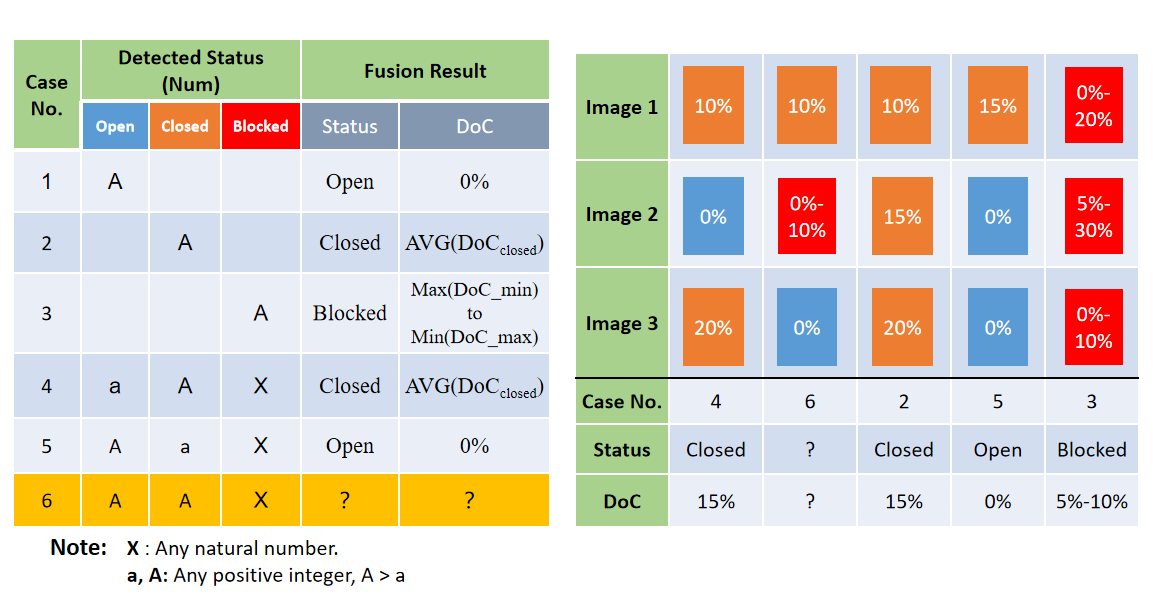
\includegraphics[width=0.9\textwidth]{Figures/Fusion.png}
  \caption{Fusion Logic Summary (Left) and an Example (Right) }
  \label{fig:14}  
\end{figure}

\chapter{Implementation}\chaplabel{4}

This chapter provides a detailed explanation of how to detect roller shutters using the PyTorch framework and the YOLOv5-v6.0 algorithm.

\section{Process Handover and Overview}

This bachelor thesis is mainly focused on detecting the status of roller shutters, while the localization of window position has been addressed in another bachelor thesis titled "Building Management: AI Mapping Image to Construction Plan" by Tao Liu. For more information regarding window localization, please refer to the aforementioned thesis. This section will also give a brief introduction of the handover process.

\begin{figure}[h]
  \centering
  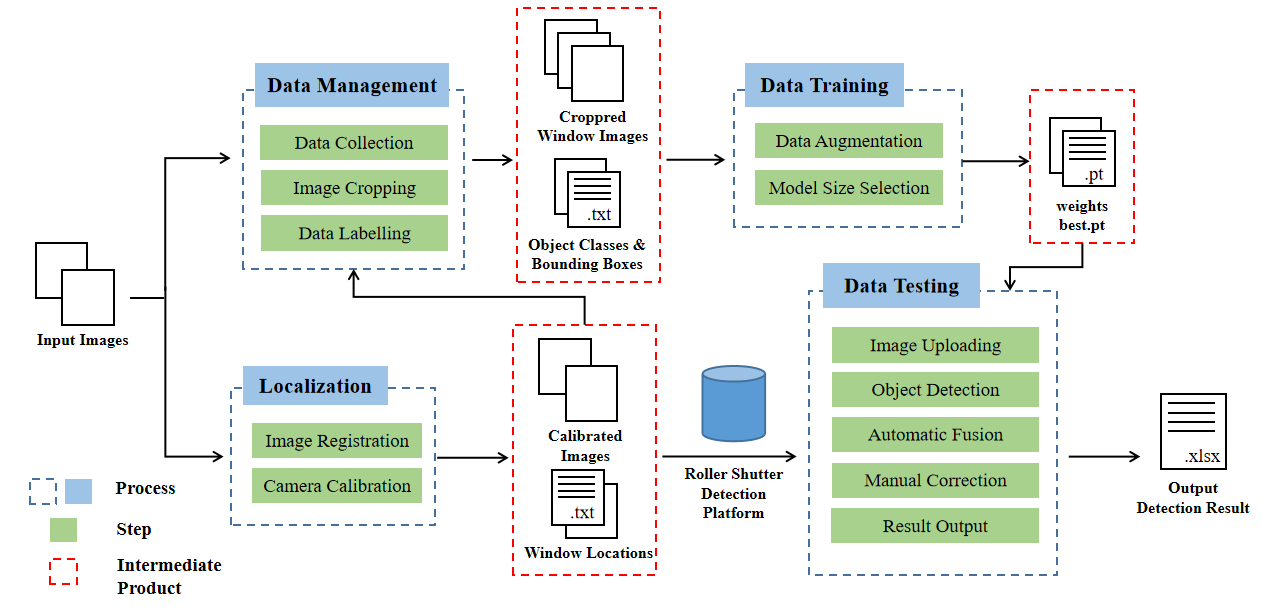
\includegraphics[width=1\textwidth]{Figures/process overview.png}
  \caption{An Overview of the Work Flow}
  \label{fig:15}  
\end{figure}

As shown in Figure \ref{fig:15}, the inputs for the entire process are building images captured by pre-set cameras on the THL campus. Tao's work involves processing these raw images into calibrated images and outputting window locations as coordinates in a text file. My work involves taking these calibrated images and window locations as inputs, and outputting the detection results, including the roller shutter status and the Degree of Closure (DoC) of each window, in an Excel file.

To enable an end-to-end process, a roller shutter detection platform is set up using the Qt Designer tool in Python, and the YOLO model is loaded for detection. Prior to loading the model, data management and data training are two critical modules for obtaining the necessary weights, which are essential for the detection model to function properly. Both raw input images and calibrated images are involved in the data collection process. These images are then manually cropped or cropped according to coordinates into separated window images for the labeling process followed. The following sections will provide a detailed explanation of each process module.

\section{Data Management}

Data Management involves three steps, which are data collection, image cropping and data labeling before adding to the training data set.

\subsection{Image Acquisition and Preprocessing}

\subsection{Labeling Strategies}


\section{Data Training}

After labeling, a text file recording the object classes and bounding boxes coordinates is generated for each cropped images. Before the training started, the model size of YOLO needs to be decided and customized data augmentation would also be an option.

\subsection{Data augmentation}

To improve the performance of detection model in different lighting conditions and robustness against occlusion. Two data augmentation methods are used, which are cutout and adjusting brightness. Cutout is the process to randomly dig out a specified number of small squares of a specified size from the image. This process can improve the robustness of the model against mild occlusions. 

\subsection{Model Selection}

\section{Data Testing and Detection Platform}

After the weights are obtained from training process, we can load this model to test its performance. In this bachelor thesis, a roller shutter detection platform is designed as the final product and evaluation tools. The following subsection will introduce its features and functions. Figure \ref{fig:16} below gives an overview of the activity flow.

\begin{figure}[h]
  \centering
  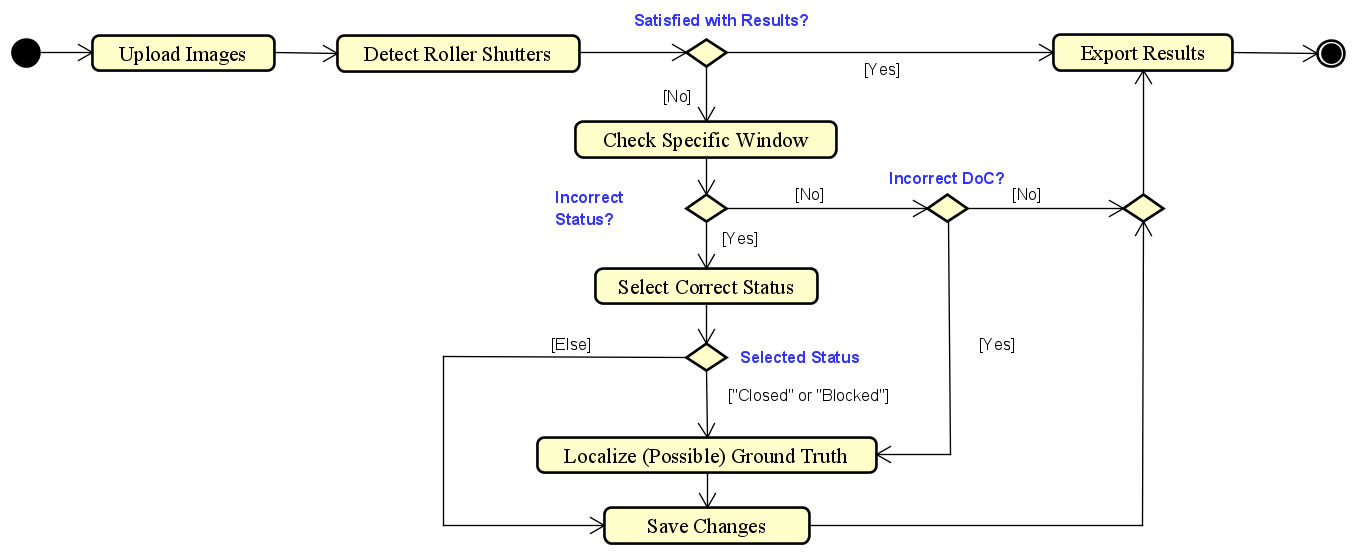
\includegraphics[width=1\textwidth]{Figures/Activity Diagram.png}
  \caption{An Overview of the Work Flow}
  \label{fig:16}  
\end{figure}

\subsection{Image Upload}


\textbf{Check Image Taken Time}

\textbf{Cropping and Warping}

\subsection{Roller Shutter Detection}

\textbf{Iterate through cropped images}

\textbf{Detect roller shutter and glass}

\textbf{Draw bounding boxes}

\subsection{Automatic Fusion}



\textbf{Fusion Logic}

\textbf{Obtain final DoC}

\subsection{Manual Correction}

\textbf{Change Status and DoC}

\subsection{Report Export}




\chapter{Evaluation and Optimization}\chaplabel{5}
\chapter{Conclusion}\chaplabel{6}

%----------------------------------------------------------------------------------------
%        THESIS CONTENT - APPENDICES
%----------------------------------------------------------------------------------------

\appendix % Cue to tell LaTeX that the following "chapters" are Appendices

% Include the appendices of the thesis as separate files from the Appendices folder
% Uncomment the lines as you write the Appendices

%\include{appendix}

%----------------------------------------------------------------------------------------
%        BIBLIOGRAPHY
%----------------------------------------------------------------------------------------


\printbibliography[title={References},heading=bibintoc,notcategory=ignore]

%----------------------------------------------------------------------------------------

\end{document}  